\section{Implementation}
In upcoming section following expressions will be used:

\begin{tabular}{ll}
$n$ & number of nodes\\
$m$ & number of edges \\
$z$ & number of zones\\
$N$ & number of path computed for one pair of zone
\end{tabular}

Transportation modelling described in previous section was implemented in Python programming language using NumPy library.

\subsection{Static shortest path search}
For determined $C$ we use Dijkstra's algorithm (complexity $O(m +n log(n) )$). So final complexity is 
$$O(z (m + n log(n)))$$
For traffic count we used also Dijkstra's algorithm. Final complexity for traffic count is 
$$O(N z (m + n log(n)))$$
For Dijkstra's algorithm we used Python library iGraph. iGraph is written in C programming language so it is quite fast. For example one Dijkstra running 30 ms ($n = 8000$ $m = 18000$).

\subsection{Data store}
All data for transportation modelling are stored in relation database PostgreSQL with extension PostGIS. PostGIS is spatial extension. Using it you can manipulate with line, point, polygon, raster.

In database there are 6 main table:

\begin{tabular}{|l|l|}
\hline
Table name & \\
\hline
\hline
\textbf{roads} & road links (edges)\\
\textbf{nodes} & nodes (vertexes)\\
\textbf{zones} & list of zones\\ 
\textbf{traffic} & \\
\textbf{general\_area\_information} & contains interested area geometry\\
\textbf{od\_pair} & Database implementation for $T$ matrix\\
\hline
\end{tabular}

In Fig \ref{img.schema} there are all table in database model and relationships between them (arrow is FOREIGN KEY).

\begin{figure}
\centering
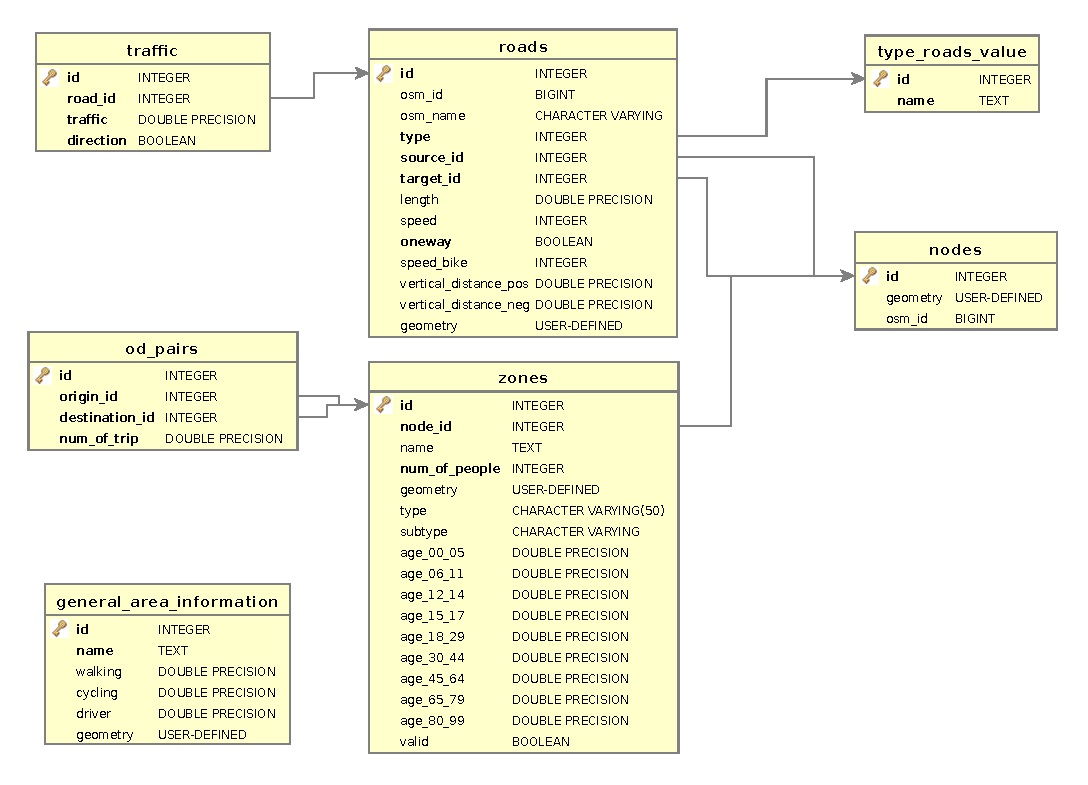
\includegraphics[width=15cm]{img/c01-transp-model/db.eps}
\caption{Database model}
\label{img.schema}
\end{figure}

More details about DB you can find in project documentation on GitHub.

\subsection{Future work}
This method of transportation modelling is very hard ($O(N z (m + n log(n)))$), so it is suitable compute this problem in some parallel environment (shared (Threads) or distributed memory (MapReduce or MPI)).

